\documentclass[11pt,a4paper]{article}

\usepackage[utf8]{inputenc}
\usepackage[T1]{fontenc}
\usepackage{mathpazo}
\usepackage[scaled=0.92]{helvet}
\usepackage[margin=1in]{geometry}
\usepackage{graphicx}
\usepackage{amsmath,amssymb,amsfonts}
\usepackage{booktabs}
\usepackage{tabularx}
\usepackage{setspace}
\usepackage{titlesec}
\usepackage{fancyhdr}
\usepackage{float}
\usepackage{caption}
\usepackage{microtype}
\usepackage{tikz}
\usepackage{xcolor}
\usepackage[hidelinks]{hyperref}

\usetikzlibrary{shapes.geometric, arrows.meta, positioning, calc, matrix, fit, backgrounds}

\setstretch{1.15}
\setlength{\parindent}{0pt}
\setlength{\parskip}{8pt}
\sloppy

\titleformat{\section}{\normalfont\large\bfseries\sffamily}{\thesection}{1em}{}
\titleformat{\subsection}{\normalfont\normalsize\bfseries\sffamily}{\thesubsection}{1em}{}
\titleformat{\subsubsection}{\normalfont\normalsize\itshape\sffamily}{\thesubsubsection}{1em}{}

\pagestyle{fancy}
\fancyhf{}
\fancyhead[L]{\small\sffamily Apa Itu Variabel? Sebuah Kajian Lintas Disiplin}
\fancyhead[R]{\small\sffamily\thepage}
\renewcommand{\headrulewidth}{0.4pt}

\captionsetup{font=small,labelfont=bf,labelsep=period}

\renewenvironment{abstract}
{\small
	\begin{center}\textbf{\sffamily Abstrak}\end{center}
	\begin{quote}}
	{\end{quote}}

\title{\vspace{-1cm}\textbf{\sffamily\LARGE Apa Itu Variabel?\\ Sebuah Kajian Komprehensif Lintas Disiplin Ilmu}}
\author{
	\textbf{Muhammad Riduwan Khafidi} \\
	\small Program Studi Teknik Rekayasa Perangkat Lunak \\
	\small Politeknik Negeri Batam \\
	\small \texttt{4342611034@students.polibatam.ac.id}
}
\date{\small\today}

\begin{document}

\maketitle
\thispagestyle{empty}

\begin{abstract}
	Istilah "variabel" (variable) merupakan salah satu konsep paling fundamental yang hadir di berbagai cabang ilmu pengetahuan, mulai dari matematika murni, ilmu komputer, hingga metodologi penelitian sosial. Meskipun terminologinya sama, esensi dan operasionalisasi variabel dapat berbeda secara signifikan antar disiplin ilmu. Makalah ini menyajikan kajian komprehensif mengenai definisi, sejarah, dan aplikasi variabel dari tiga perspektif utama. Dalam matematika, variabel dibahas sebagai simbol abstrak yang merepresentasikan objek atau nilai yang tidak diketahui. Dalam ilmu komputer, variabel dipahami sebagai abstraksi lokasi penyimpanan yang dipasangkan dengan nama simbolik, di mana pada beberapa bahasa modern (seperti Rust) konsep ini lebih tepat disebut sebagai binding. Sementara dalam penelitian, variabel dipahami sebagai representasi operasional dari sebuah atribut yang memiliki level pengukuran tertentu. Melalui penelusuran literatur dan sembilan visualisasi konseptual, makalah ini bertujuan untuk memberikan pemahaman holistik mengenai bagaimana satu konsep dapat berevolusi dan diadaptasi sesuai dengan kebutuhan spesifik masing-masing bidang keilmuan.
\end{abstract}

\section{Pendahuluan}

\subsection{Latar Belakang}

Dalam setiap upaya manusia untuk memahami dan memanipulasi dunia, baik dunia abstrak dari angka dan logika, dunia digital dari perangkat lunak, maupun dunia nyata dari fenomena sosial, manusia membutuhkan alat untuk merepresentasikan informasi. Alat tersebut dikenal dengan sebutan variabel. Secara etimologis, kata "variabel" berasal dari bahasa Latin \textit{variabilis} yang berarti "dapat berubah" \cite{wikipedia_math}. Namun seiring dengan perkembangan peradaban dan lahirnya disiplin-disiplin ilmu baru, makna dan peran variabel telah mengalami metamorfosis yang panjang.

\subsection{Tiga Perspektif yang Dibahas}

Makalah ini membedah konsep variabel dari tiga kacamata yang berbeda. Gambar~\ref{fig:overview} merangkum ketiganya secara visual.

\begin{figure}[H]
	\centering
	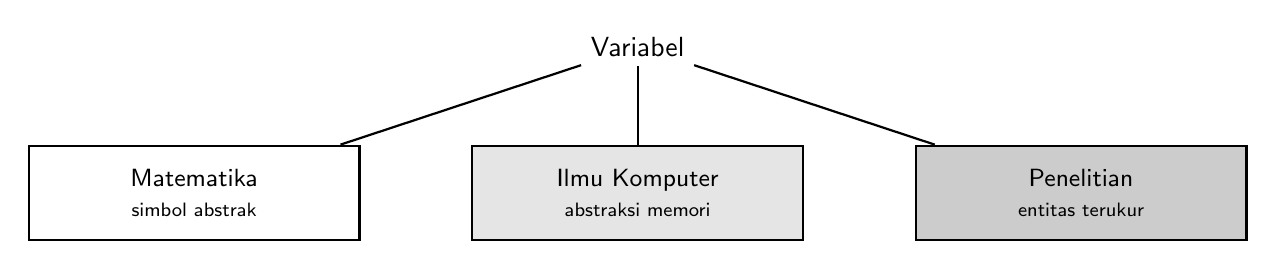
\begin{tikzpicture}[
			node distance=0.5cm,
			cat/.style={rectangle, draw=black, thick, minimum width=4.2cm, minimum height=1.2cm, align=center, font=\sffamily\small},
			line/.style={draw, thick}
		]
		\node[font=\sffamily] (root) at (0, 1.5) {Variabel};
		\node[cat, fill=white, below left=1cm and 2.8cm of root] (math) {Matematika \\ \scriptsize simbol abstrak};
		\node[cat, fill=black!10, below=1cm of root] (cs) {Ilmu Komputer \\ \scriptsize abstraksi memori};
		\node[cat, fill=black!20, below right=1cm and 2.8cm of root] (res) {Penelitian \\ \scriptsize entitas terukur};

		\draw[line] (root) -- (math);
		\draw[line] (root) -- (cs);
		\draw[line] (root) -- (res);
	\end{tikzpicture}
	\caption{Tiga perspektif variabel yang dibahas dalam makalah ini.}
	\label{fig:overview}
\end{figure}

Bagian kedua membahas variabel dalam ranah matematika, menelusuri jejak sejarahnya dari peradaban Mesir Kuno hingga notasi modern. Bagian ketiga berfokus pada variabel dalam ilmu komputer, di mana variabel berfungsi sebagai entitas yang menjembatani logika manusia dengan memori mesin. Bagian keempat mengupas bagaimana variabel didefinisikan dan dioperasionalisasikan dalam konteks penelitian ilmiah. Bagian kelima menyandingkan ketiganya dalam satu tabel perbandingan.

\section{Variabel dalam Perspektif Matematika}

\subsection{Definisi Dasar}

Dalam matematika, variabel didefinisikan sebagai sebuah simbol, biasanya berupa huruf, yang merujuk pada suatu objek matematika yang tidak ditentukan secara spesifik \cite{sobolev}. Penggunaan simbol ini memungkinkan matematikawan merumuskan persamaan dan generalisasi yang berlaku universal, terlepas dari nilai spesifik yang mungkin dimiliki variabel tersebut.

\subsection{Sejarah Notasi: Dari Aha hingga Descartes}

Sejarah penggunaan variabel dalam matematika sangat panjang. Jejak paling awal dapat ditelusuri hingga peradaban Mesir Kuno sekitar tahun 1500 SM melalui \textit{Moscow Mathematical Papyrus} dan \textit{Rhind Mathematical Papyrus}. Pada masa itu, masalah-masalah matematika yang melibatkan kuantitas tidak diketahui dijelaskan secara retoris, dikenal sebagai "Aha problems" \cite{wikipedia_math}. Kuantitas tersebut disebut \textit{aha} atau "tumpukan".

Memasuki era Yunani Kuno, karya seperti \textit{Elements} karya Euklid (sekitar 300 SM) mendeskripsikan matematika secara geometris. Pada abad ke-3 Masehi, Diophantus dari Alexandria memperkenalkan bentuk awal aljabar sinkopasi dalam \textit{Arithmetica} \cite{boyer}. Diophantus menggunakan simbol khusus untuk variabel yang tidak diketahui, meskipun belum memiliki simbol untuk operasi dan relasi seperti sekarang.

Notasi modern baru muncul pada akhir abad ke-16 dan awal abad ke-17. François Viète memperkenalkan ide merepresentasikan angka yang diketahui dan tidak diketahui dengan huruf. Konvensi ini disempurnakan oleh René Descartes pada 1637, yang memperkenalkan kebiasaan menggunakan huruf akhir alfabet seperti \(x\), \(y\), dan \(z\) untuk variabel, serta huruf awal seperti \(a\), \(b\), dan \(c\) untuk konstanta \cite{wikipedia_math}. Gambar~\ref{fig:math-timeline} merangkum rentang sejarah tersebut.

\begin{figure}[H]
	\centering
	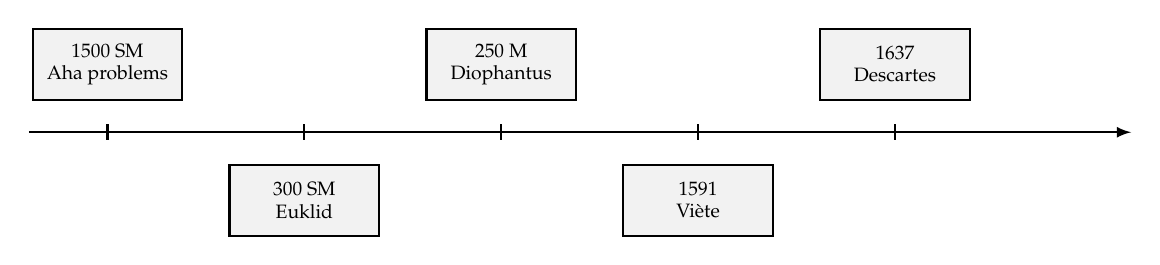
\begin{tikzpicture}[
			ev/.style={rectangle, draw=black, thick, fill=black!5, minimum width=1.9cm, minimum height=0.9cm, align=center, font=\scriptsize},
			line/.style={draw, thick}
		]
		\draw[line, -latex] (-7, 0) -- (7, 0);

		\draw[thick] (-6, 0.1) -- (-6, -0.1);
		\node[ev, above=0.2cm] at (-6, 0.2) {1500 SM \\ Aha problems};

		\draw[thick] (-3.5, 0.1) -- (-3.5, -0.1);
		\node[ev, below=0.2cm] at (-3.5, -0.2) {300 SM \\ Euklid};

		\draw[thick] (-1, 0.1) -- (-1, -0.1);
		\node[ev, above=0.2cm] at (-1, 0.2) {250 M \\ Diophantus};

		\draw[thick] (1.5, 0.1) -- (1.5, -0.1);
		\node[ev, below=0.2cm] at (1.5, -0.2) {1591 \\ Vi\`ete};

		\draw[thick] (4, 0.1) -- (4, -0.1);
		\node[ev, above=0.2cm] at (4, 0.2) {1637 \\ Descartes};
	\end{tikzpicture}
	\caption{Timeline evolusi notasi variabel dalam matematika.}
	\label{fig:math-timeline}
\end{figure}

\subsection{Tiga Peran Variabel}

Dalam perkembangan selanjutnya, variabel matematika dapat memainkan beberapa peran berbeda. Gambar~\ref{fig:roles-math} membedakan tiga peran yang paling sering muncul.

\begin{figure}[H]
	\centering
	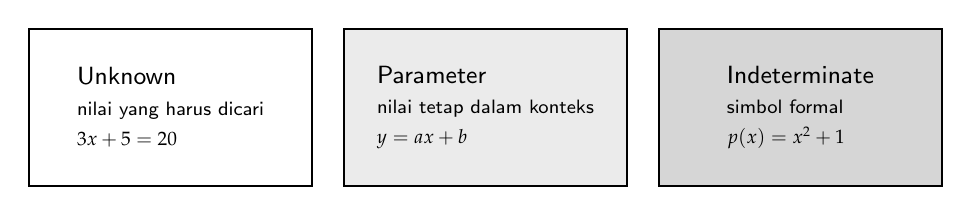
\begin{tikzpicture}[
			box/.style={rectangle, draw=black, thick, minimum width=3.6cm, minimum height=2cm, align=left, font=\sffamily\small, inner sep=8pt}
		]
		\node[box, fill=white] (u) at (-4, 0) {
			Unknown \\
			\scriptsize nilai yang harus dicari \\
			\scriptsize \(3x + 5 = 20\)
		};
		\node[box, fill=black!8] (p) at (0, 0) {
			Parameter \\
			\scriptsize nilai tetap dalam konteks \\
			\scriptsize \(y = ax + b\)
		};
		\node[box, fill=black!16] (i) at (4, 0) {
			Indeterminate \\
			\scriptsize simbol formal \\
			\scriptsize \(p(x) = x^2 + 1\)
		};
	\end{tikzpicture}
	\caption{Tiga peran variabel dalam matematika.}
	\label{fig:roles-math}
\end{figure}

Unknown adalah nilai yang harus ditemukan agar persamaan menjadi benar. Parameter adalah nilai yang dianggap tetap selama proses penyelesaian masalah tertentu. Indeterminate adalah simbol formal yang dipakai dalam polinomial atau deret pangkat, bukan untuk dicari nilainya, melainkan untuk mendefinisikan struktur objek matematika itu sendiri \cite{wikipedia_math}.

\subsection{Pergeseran ke Formalisme Abad ke-19}

Memasuki abad ke-19, Karl Weierstrass memperkenalkan formalisme baru yang mengubah pemahaman intuitif tentang "limit" (di mana variabel dianggap bergerak mendekati suatu nilai) menjadi definisi statis yang ketat. Sejak saat itu, pemahaman modern terhadap variabel matematika bergeser menjadi sekadar simbol yang merepresentasikan objek matematika tidak diketahui atau dapat digantikan oleh elemen dari himpunan tertentu \cite{wikipedia_math}.

\section{Variabel dalam Ilmu Komputer}

\subsection{Definisi dan Konsep Binding}

Berbeda dengan matematika yang memperlakukan variabel sebagai konsep abstrak, ilmu komputer, khususnya bahasa pemrograman tingkat tinggi, mendefinisikan variabel sebagai abstraksi lokasi penyimpanan yang dipasangkan dengan nama simbolik \cite{brookshear,wikipedia_cs}. Representasi variabel di memori bergantung pada bahasa pemrogramannya. Pada bahasa seperti C atau C++, variabel biasanya merepresentasikan alamat memori spesifik dan membutuhkan kompilator untuk menggantikan nama simbolik dengan alamat tersebut. Pada bahasa dinamis seperti Python atau Ruby, variabel lebih tepat dipandang sebagai nama yang diasosiasikan dengan suatu objek, dan alokasi memori ditangani secara transparan oleh runtime \cite{wikipedia_cs}.

Dalam konteks bahasa pemrograman modern seperti Rust, istilah yang lebih tepat untuk variabel adalah binding, yaitu proses mengikat sebuah nama ke sebuah nilai \cite{klabnik}. Gambar~\ref{fig:komputer_memori} mengilustrasikan konsep tersebut.

\begin{figure}[H]
	\centering
	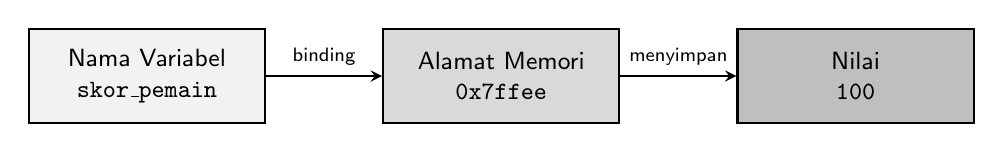
\begin{tikzpicture}[
			box/.style={rectangle, draw=black, thick, minimum width=3cm, minimum height=1.2cm, align=center, font=\sffamily\small},
			arrow/.style={->, >=stealth, thick}
		]
		\node[box, fill=black!5] (nama) at (0,0) {Nama Variabel \\ \texttt{skor\_pemain}};
		\node[box, fill=black!15] (alamat) at (4.5,0) {Alamat Memori \\ \texttt{0x7ffee}};
		\node[box, fill=black!25] (nilai) at (9,0) {Nilai \\ \texttt{100}};

		\draw[arrow] (nama) -- (alamat) node[midway, above, font=\scriptsize\sffamily] {binding};
		\draw[arrow] (alamat) -- (nilai) node[midway, above, font=\scriptsize\sffamily] {menyimpan};
	\end{tikzpicture}
	\caption{Konsep binding dan alokasi memori pada variabel ilmu komputer.}
	\label{fig:komputer_memori}
\end{figure}

\subsection{Scope dan Extent}

Atribut penting dari sebuah variabel dalam ilmu komputer terbagi menjadi beberapa aspek. Aspek pertama adalah scope (ruang lingkup) dan extent (jangka waktu). Scope mendefinisikan di mana teks program variabel dapat diakses, sedangkan extent mendefinisikan kapan dalam waktu eksekusi variabel tersebut memiliki nilai yang bermakna. Gambar~\ref{fig:scope} menunjukkan tiga variabel yang memiliki nama sama tetapi scope berbeda.

\begin{figure}[H]
	\centering
	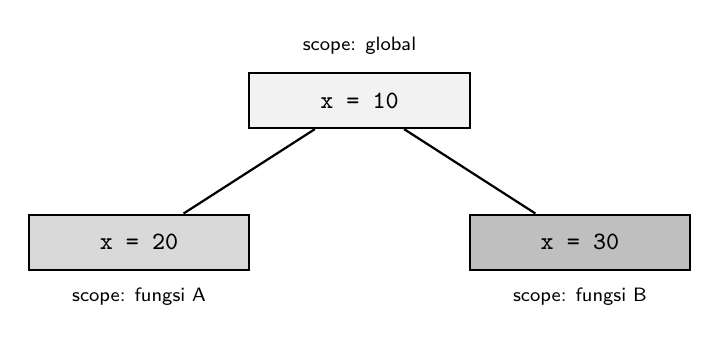
\begin{tikzpicture}[
			box/.style={rectangle, draw=black, thick, minimum width=2.8cm, minimum height=0.7cm, font=\ttfamily\small, align=center}
		]
		\node[box, fill=black!5] (g) at (0, 0) {x = 10};
		\node[font=\scriptsize\sffamily, above=0.1cm of g] {scope: global};

		\node[box, fill=black!15] (a) at (-2.8, -1.8) {x = 20};
		\node[font=\scriptsize\sffamily, below=0.1cm of a] {scope: fungsi A};

		\node[box, fill=black!25] (b) at (2.8, -1.8) {x = 30};
		\node[font=\scriptsize\sffamily, below=0.1cm of b] {scope: fungsi B};

		\draw[thick] (g) -- (a);
		\draw[thick] (g) -- (b);
	\end{tikzpicture}
	\caption{Tiga variabel bernama \texttt{x} dengan scope berbeda.}
	\label{fig:scope}
\end{figure}

Berdasarkan masa hidupnya, variabel dapat diklasifikasikan menjadi static variable (dialokasikan sebelum eksekusi dan tetap ada), stack-dynamic variable (dialokasikan saat fungsi dipanggil), explicit heap-dynamic variable (dialokasikan manual oleh pemrogram), dan implicit heap-dynamic variable (dialokasikan otomatis saat nilai diikatkan) \cite{wikipedia_cs}.

\subsection{Static versus Dynamic Typing}

Aspek kedua adalah typing (tipe data). Dalam bahasa dengan tipe statis seperti C atau Rust, variabel terikat pada tipe data tertentu, dan pelanggaran tipe tertangkap saat kompilasi. Dalam bahasa dengan tipe dinamis seperti Python, tipe data melekat pada nilai atau objek, bukan pada nama variabelnya. Sebuah nama variabel dapat diikat ulang ke objek dengan tipe berbeda. Gambar~\ref{fig:typing} membandingkan keduanya.

\begin{figure}[H]
	\centering
	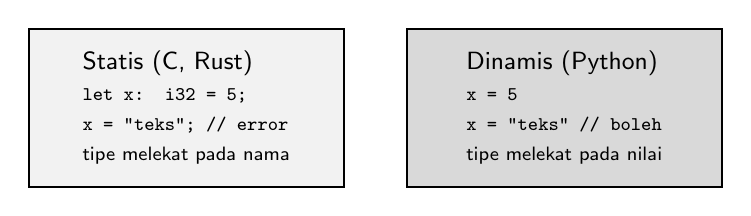
\begin{tikzpicture}[
			box/.style={rectangle, draw=black, thick, minimum width=4cm, minimum height=1.8cm, align=left, font=\sffamily\small, inner sep=8pt}
		]
		\node[box, fill=black!5] at (-2.4, 0) {
			Statis (C, Rust) \\
			\ttfamily\scriptsize let x: i32 = 5; \\
			\ttfamily\scriptsize x = "teks"; // error \\
			\scriptsize tipe melekat pada nama
		};
		\node[box, fill=black!15] at (2.4, 0) {
			Dinamis (Python) \\
			\ttfamily\scriptsize x = 5 \\
			\ttfamily\scriptsize x = "teks" // boleh \\
			\scriptsize tipe melekat pada nilai
		};
	\end{tikzpicture}
	\caption{Perbedaan tipe statis dan tipe dinamis pada variabel.}
	\label{fig:typing}
\end{figure}

\subsection{Aliasing}

Aspek terakhir adalah fenomena aliasing, yaitu situasi di mana satu lokasi penyimpanan yang sama dapat dirujuk oleh beberapa identifier berbeda. Ini umum terjadi pada passing by reference, pointer, atau variabel yang menunjuk objek yang sama. Gambar~\ref{fig:aliasing} mengilustrasikannya.

\begin{figure}[H]
	\centering
	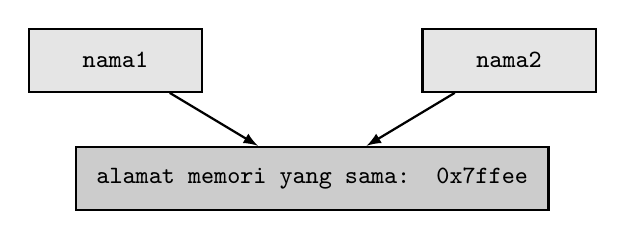
\begin{tikzpicture}[
			box/.style={rectangle, draw=black, thick, minimum width=2.2cm, minimum height=0.8cm, font=\ttfamily\small, align=center}
		]
		\node[box, fill=black!10] (a) at (-2.5, 0) {nama1};
		\node[box, fill=black!10] (b) at (2.5, 0) {nama2};
		\node[box, fill=black!20, minimum width=6cm] (mem) at (0, -1.5) {alamat memori yang sama: \texttt{0x7ffee}};

		\draw[thick, -latex] (a) -- (mem);
		\draw[thick, -latex] (b) -- (mem);
	\end{tikzpicture}
	\caption{Aliasing: dua nama merujuk ke lokasi memori yang sama.}
	\label{fig:aliasing}
\end{figure}

Perubahan nilai melalui \texttt{nama1} akan terlihat melalui \texttt{nama2}, karena keduanya merujuk ke lokasi yang sama. Selain aliasing, parameter formal pada sebuah fungsi juga dikategorikan sebagai variabel yang ruang lingkupnya terbatas pada fungsi tersebut \cite{wikipedia_cs}.

\section{Variabel dalam Metodologi Penelitian}

\subsection{Atribut dan Variabel}

Dalam dunia penelitian ilmiah, khususnya ilmu sosial dan statistik, pemahaman mengenai variabel bergeser dari sekadar simbol atau lokasi memori menjadi entitas konseptual yang dapat diukur. Di sini, konsep variabel sangat erat kaitannya dengan "atribut". Menurut Earl R. Babbie dalam bukunya \textit{The Practice of Social Research}, sebuah atribut adalah kualitas atau karakteristik yang melekat pada suatu objek (misalnya seseorang bisa memiliki atribut "pria", "tinggi", atau "konservatif"). Sementara itu, variabel adalah kumpulan logis dari atribut-atribut tersebut \cite{babbie,wikipedia_research}. Gambar~\ref{fig:attr-var} mengilustrasikan hubungan tersebut.

\begin{figure}[H]
	\centering
	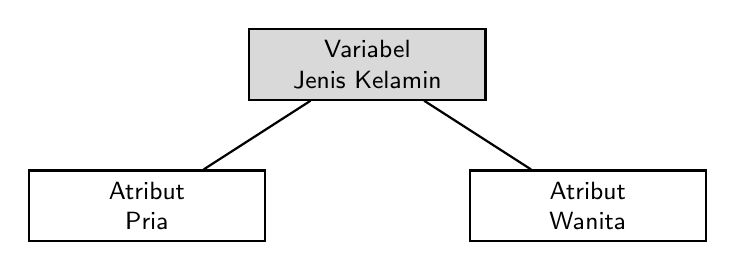
\begin{tikzpicture}[
			box/.style={rectangle, draw=black, thick, minimum width=3cm, minimum height=0.9cm, font=\sffamily\small, align=center}
		]
		\node[box, fill=black!15] (var) at (0, 0) {Variabel \\ Jenis Kelamin};
		\node[box, fill=white] (a1) at (-2.8, -1.8) {Atribut \\ Pria};
		\node[box, fill=white] (a2) at (2.8, -1.8) {Atribut \\ Wanita};

		\draw[thick] (var) -- (a1);
		\draw[thick] (var) -- (a2);
	\end{tikzpicture}
	\caption{Variabel sebagai himpunan atribut.}
	\label{fig:attr-var}
\end{figure}

Variabel dikatakan "bervariasi" karena nilai atau atributnya bisa berbeda-beda antar objek yang diteliti. Perbedaan mendasar antara atribut dan variabel terletak pada tingkat operasionalisasinya. Atribut sering bersifat intuitif, sedangkan variabel adalah cara operasional di mana atribut tersebut direpresentasikan untuk keperluan pemrosesan data lebih lanjut \cite{wikipedia_research}.

\subsection{Empat Level Pengukuran}

Nilai dari setiap variabel secara statistik terdistribusi di sepanjang domain variabel tersebut. Domain adalah himpunan semua nilai yang mungkin dimiliki sebuah variabel. Dalam metodologi penelitian, level pengukuran variabel secara garis besar dibagi menjadi empat, seperti pada Gambar~\ref{fig:levels} \cite{babbie}.

\begin{figure}[H]
	\centering
	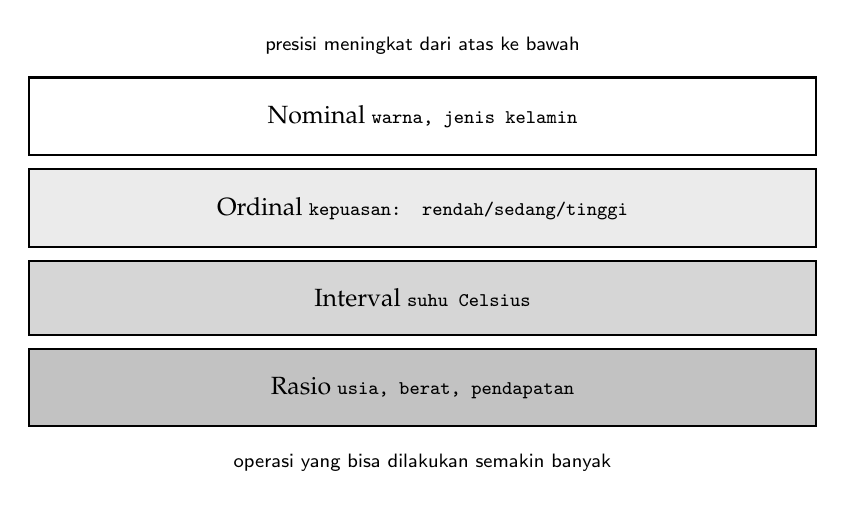
\begin{tikzpicture}[
			lvl/.style={rectangle, draw=black, thick, minimum width=10cm, minimum height=0.8cm, font=\small, align=left, inner sep=10pt}
		]
		\node[font=\scriptsize\sffamily] at (0, 0.9) {presisi meningkat dari atas ke bawah};
		\node[lvl, fill=white] (n) at (0, 0) {Nominal \hfill \ttfamily\scriptsize warna, jenis kelamin};
		\node[lvl, fill=black!8, below=0.15cm of n] (o) {Ordinal \hfill \ttfamily\scriptsize kepuasan: rendah/sedang/tinggi};
		\node[lvl, fill=black!16, below=0.15cm of o] (i) {Interval \hfill \ttfamily\scriptsize suhu Celsius};
		\node[lvl, fill=black!24, below=0.15cm of i] (r) {Rasio \hfill \ttfamily\scriptsize usia, berat, pendapatan};
		\node[font=\scriptsize\sffamily] at (0, -4.4) {operasi yang bisa dilakukan semakin banyak};
	\end{tikzpicture}
	\caption{Empat level pengukuran variabel.}
	\label{fig:levels}
\end{figure}

Level nominal hanya membedakan kategori tanpa urutan, seperti warna atau jenis kelamin. Level ordinal menambahkan urutan, seperti tingkat kepuasan. Level interval menambahkan jarak bermakna tanpa titik nol absolut, seperti suhu Celsius. Level rasio menambahkan titik nol absolut, seperti berat, usia, dan pendapatan. Sebagai contoh konkret, "usia" dapat didikotomikan menjadi "muda" dan "tua" (nominal), diurutkan menjadi "muda", "paruh baya", "tua" (ordinal), atau direpresentasikan sebagai angka 20, 21, 22 tahun (rasio) \cite{wikipedia_research}.

\subsection{Peran Variabel dalam Sebab-Akibat}

Selain level pengukuran, penelitian juga mengenal peran variabel dalam hubungan sebab-akibat. Variabel independen adalah variabel yang mempengaruhi atau menjadi sebab perubahan variabel lainnya. Variabel dependen adalah variabel yang dipengaruhi atau menjadi akibat. Variabel kontrol adalah variabel yang dianggap konstan atau dikendalikan oleh peneliti agar tidak mengganggu hubungan antara variabel independen dan dependen \cite{babbie}. Gambar~\ref{fig:roles-research} menampilkan ketiganya.

\begin{figure}[H]
	\centering
	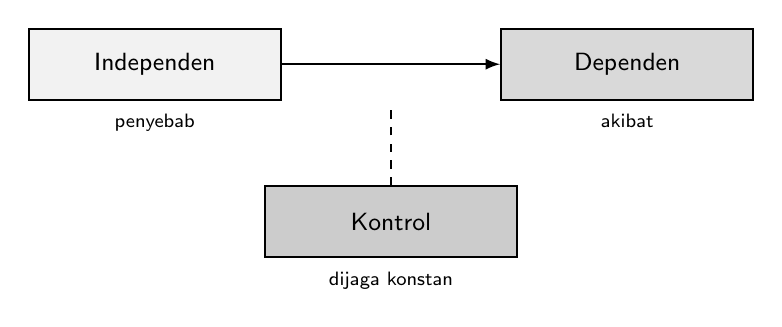
\begin{tikzpicture}[
			box/.style={rectangle, draw=black, thick, minimum width=3.2cm, minimum height=0.9cm, font=\sffamily\small, align=center},
			arr/.style={draw, thick, -latex}
		]
		\node[box, fill=black!5] (ind) at (0, 0) {Independen};
		\node[font=\scriptsize\sffamily, below=0.05cm of ind] {penyebab};

		\node[box, fill=black!15] (dep) at (6, 0) {Dependen};
		\node[font=\scriptsize\sffamily, below=0.05cm of dep] {akibat};

		\node[box, fill=black!20] (ctrl) at (3, -2) {Kontrol};
		\node[font=\scriptsize\sffamily, below=0.05cm of ctrl] {dijaga konstan};

		\draw[arr] (ind) -- (dep);
		\draw[thick, dashed] (ctrl) -- (3, -0.5);
	\end{tikzpicture}
	\caption{Peran variabel dalam hubungan sebab-akibat.}
	\label{fig:roles-research}
\end{figure}

\section{Perbandingan Lintas Disiplin}

Setelah menelusuri ketiga perspektif, perbedaan dan persamaan antar disiplin dapat diringkas dalam satu tabel. Tabel~\ref{tab:comparison} menyandingkannya secara berdampingan.

\begin{table}[H]
	\centering
	\caption{Perbandingan konsep variabel lintas disiplin.}
	\label{tab:comparison}
	\footnotesize
	\begin{tabularx}{\textwidth}{l X X X}
		\toprule
		Aspek           & Matematika                            & Ilmu Komputer                        & Penelitian                            \\
		\midrule
		Definisi        & simbol yang mewakili objek matematika & abstraksi lokasi penyimpanan bernama & representasi operasional dari atribut \\
		Wujud           & tulisan di kertas                     & slot di memori                       & entri di lembar data                  \\
		Kebebasan nilai & tidak ditentukan hingga disubstitusi  & terikat saat eksekusi                & terdistribusi di dalam domain         \\
		Operasi utama   & substitusi dan penyelesaian           & pembacaan dan penulisan              & pengukuran dan analisis               \\
		Fokus           & generalisasi pola                     & efisiensi memori dan tipe            & operasionalisasi konsep               \\
		Satuan waktu    & tidak relevan                         & extent dan lifetime                  & tidak relevan                         \\
		Kesalahan lazim & substitusi keliru                     & tipe tidak cocok                     & level pengukuran salah                \\
		\bottomrule
	\end{tabularx}
\end{table}

Tiga kesamaan yang menonjol dari ketiganya. Pertama, ketiganya memakai satu nama simbolik untuk merujuk pada sesuatu yang lebih kompleks di baliknya. Kedua, ketiganya membatasi nilai yang boleh diambil, entah lewat domain himpunan, tipe data, atau level pengukuran. Ketiga, ketiganya menjadikan variabel sebagai alat untuk mengelola kompleksitas informasi.

\section{Kesimpulan}

Berdasarkan pembahasan di atas, dapat disimpulkan bahwa variabel adalah sebuah konsep yang beradaptasi dengan lingkungan disiplin ilmunya. Dalam matematika, variabel adalah simbol murni yang merepresentasikan nilai tak diketahui, yang notasi dan sejarahnya telah berevolusi selama ribuan tahun. Dalam ilmu komputer, variabel adalah abstraksi yang pada saat runtime dipetakan ke lokasi penyimpanan atau nilai tertentu, dan representasinya di memori bergantung pada bahasa serta implementasinya. Dalam metodologi penelitian, variabel adalah jembatan operasional yang menghubungkan konsep teoretis (atribut) dengan data empiris yang dapat diukur dan dianalisis secara statistik.

Meskipun terdapat perbedaan mendasar dalam cara pandang terhadap variabel, ketiga disiplin ilmu ini memiliki satu kesamaan: variabel digunakan sebagai alat fundamental untuk mengelola kompleksitas informasi, baik informasi abstrak dalam bentuk persamaan, informasi biner dalam bentuk data digital, maupun informasi empiris dalam bentuk data penelitian. Dengan memahami ketiga perspektif ini secara bersamaan, seorang pembelajar dapat membaca literatur lintas disiplin tanpa kebingungan terminologi, dan dapat memilih cara pandang yang paling sesuai dengan masalah yang sedang dihadapi.

\newpage
\section*{Referensi}
\addcontentsline{toc}{section}{Referensi}

\begin{thebibliography}{99}

	\bibitem{babbie}
	Babbie, E. R. (2009). \textit{The Practice of Social Research} (12th ed.). Wadsworth Publishing.

	\bibitem{boyer}
	Boyer, C. B. (1991). \textit{A History of Mathematics}. John Wiley \& Sons.

	\bibitem{brookshear}
	Brookshear, J. G. (2019). \textit{Computer Science: An Overview} (13th ed.). Pearson.

	\bibitem{klabnik}
	Klabnik, S., \& Nichols, C. (2019). \textit{The Rust Programming Language}. No Starch Press.

	\bibitem{sobolev}
	Sobolev, S. K. (n.d.). Individual variable. In \textit{Encyclopedia of Mathematics}. Springer. Diakses dari \url{http://encyclopediaofmath.org/index.php?title=Individual_variable}

	\bibitem{wikipedia_cs}
	Wikipedia Contributors. (2026, October 30). \textit{Variable (high-level programming language)}. Wikipedia, The Free Encyclopedia. Diakses dari \url{https://en.wikipedia.org/wiki/Variable_(high-level_programming_language)}

	\bibitem{wikipedia_math}
	Wikipedia Contributors. (2026, October 3). \textit{Variable (mathematics)}. Wikipedia, The Free Encyclopedia. Diakses dari \url{https://en.wikipedia.org/wiki/Variable_(mathematics)}

	\bibitem{wikipedia_research}
	Wikipedia Contributors. (2026, May 8). \textit{Variable and attribute (research)}. Wikipedia, The Free Encyclopedia. Diakses dari \url{https://en.wikipedia.org/wiki/Variable_and_attribute_(research)}

\end{thebibliography}

\end{document}
